\chapter{Process Discovery and Alpha Algorithm}
    
    One of the main challenges with process discovery is that the model derived from event logs may not capture the entire behavior of the underlying real process. This is because the real process is hidden from us, and we only observe the cases recorded in the event log—typically only the successful cases. As a result, we need to apply some abstraction techniques to generalize the model beyond the observed cases.
    
    In Petri nets, we aim to impose restrictions, for example, on the order of events. To achieve this, we introduce \textit{places} that control the firing of transitions. However, this can lead to \textbf{overfitting}, if we add too many places, or \textbf{underfitting}, if we add too few places. The addition of even a single place can eliminate some transitions from the net, leading to the exclusion of potential behaviors.
    
    \section{Alpha Algorithm}
    The Alpha Algorithm provides a systematic way to discover a process model from event logs by leveraging the relationships between activities. To understand these relationships, we define the following operators:
    \begin{itemize}
        \item \textbf{Direct succession (\(>\)):} Activity \(x > y\) if \(x\) is directly followed by \(y\) in some case.
        \item \textbf{Causality (\(\rightarrow\)):} Activity \(x \rightarrow y\) if \(x > y\) and not \(y > x\).
        \item \textbf{Parallel (\(||\)):} Activity \(x || y\) if \(x > y\) and \(y > x\), indicating that they can occur in parallel.
        \item \textbf{Choice (\(\#\)):} Activity \(x \# y\) if neither \(x > y\) nor \(y > x\), indicating a choice between the two. If $x\#y$ then $y\#x$.
    \end{itemize}
    
    With these operators, we can construct basic patterns in process models:
    
    \subsection{Sequence Pattern}
    The sequence pattern is represented as \(a \rightarrow b\), meaning that activity \(b\) always occurs after activity \(a\).
    
    \begin{center}
        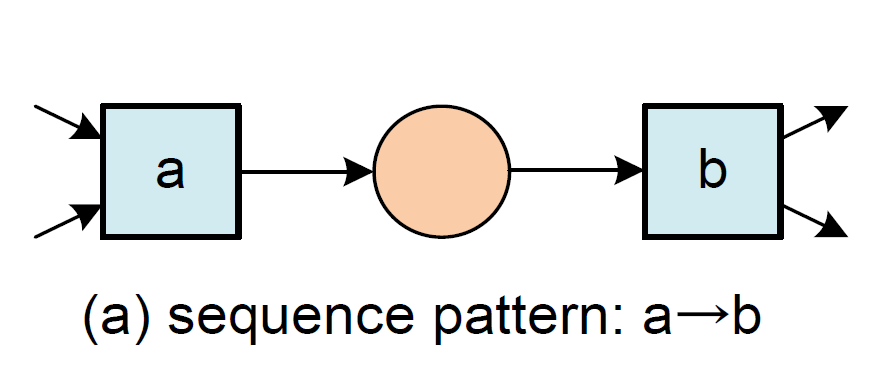
\includegraphics[width=0.5\textwidth]{capitolo 5/5 sequence pattern.png}
    \end{center}
    
    \subsection{XOR-Split Pattern}
    The XOR-split pattern is represented as \(a \rightarrow b\), \(a \rightarrow c\), and \(b \# c\), indicating that after activity \(a\), either \(b\) or \(c\) will follow, but not both.
    
    \begin{center}
        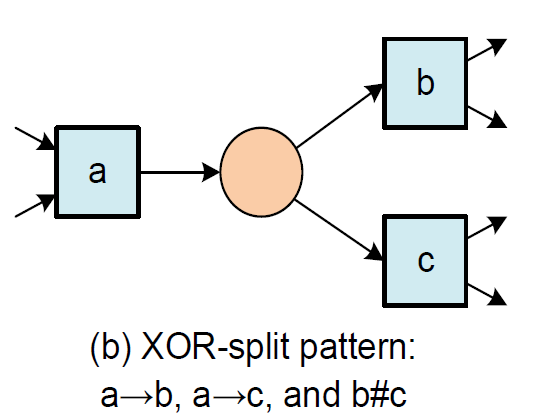
\includegraphics[width=0.5\textwidth]{capitolo 5/5 xor split.png}
    \end{center}
    
    \subsection{XOR-Join Pattern}
    The XOR-join pattern is represented as \(a \rightarrow c\), \(b \rightarrow c\), and \(a \# b\), meaning that activity \(c\) can be reached from either \(a\) or \(b\), but \(a\) and \(b\) are mutually exclusive.
    
    \begin{center}
        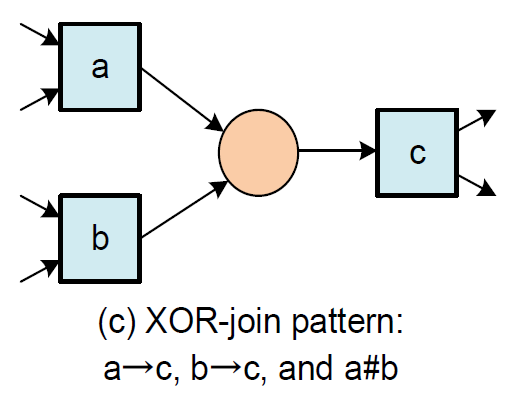
\includegraphics[width=0.5\textwidth]{capitolo 5/5 xor join.png}
    \end{center}
    
    \subsection{AND-Split Pattern}
    The AND-split pattern is represented as \(a \rightarrow b\), \(a \rightarrow c\), and \(b || c\), indicating that after activity \(a\), both \(b\) and \(c\) will occur in parallel.
    
    \begin{center}
        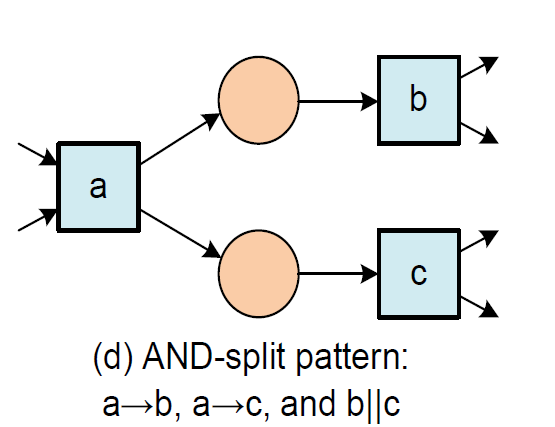
\includegraphics[width=0.5\textwidth]{capitolo 5/5 and split pattern.png}
    \end{center}
    
    \subsection{AND-Join Pattern}
    The AND-join pattern is represented as \(a \rightarrow c\), \(b \rightarrow c\), and \(a || b\), meaning that activity \(c\) occurs after both \(a\) and \(b\) have completed.
    
    \begin{center}
        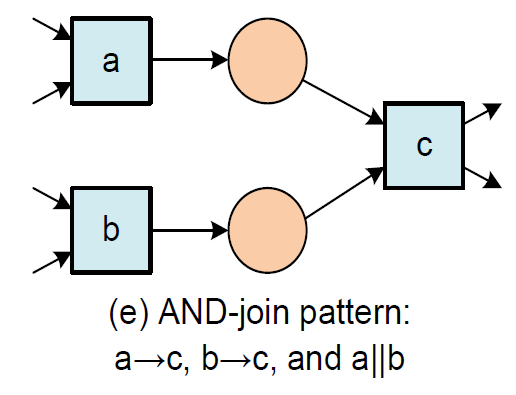
\includegraphics[width=0.5\textwidth]{capitolo 5/5 and join pattern.png}
    \end{center}
    
    \subsection{Summary of Patterns}
    The following image summarizes all the patterns described above:
    
    \begin{center}
        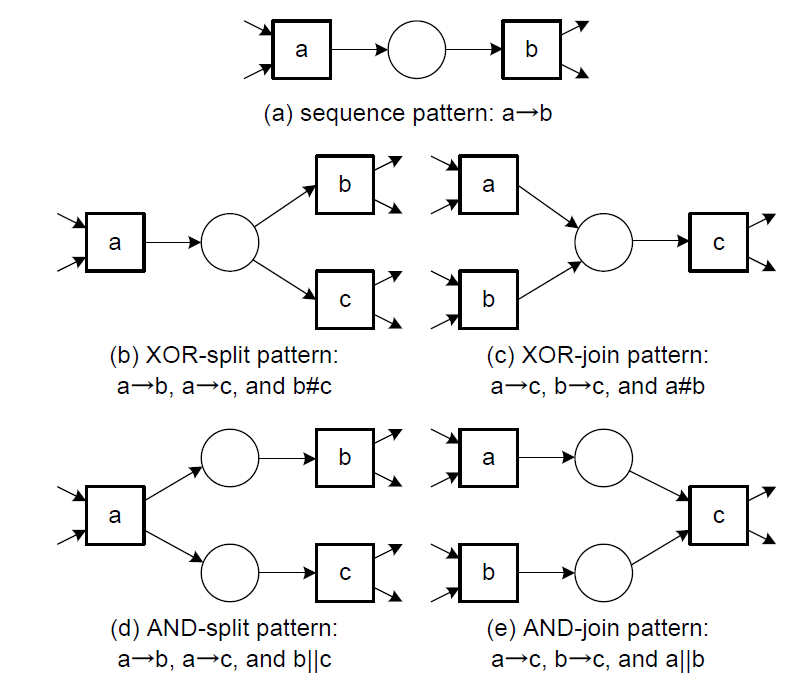
\includegraphics[width=\textwidth]{capitolo 5/5 recap pattern.png}
    \end{center}
    
    \section{Steps of the Alpha Algorithm}
    
    Given an event log \(L\) over a set of transitions \(T\) and trace $\sigma$, the Alpha Algorithm, $\alpha(L)$, defines a workflow model in the following steps:
    
    \begin{enumerate}
        \item Define the set \(T_L\) as the set of all transitions in \(L\): \[
        T_L = \{ t \in T \mid \exists \sigma \in L \text{ such that } t \in \sigma \}.
        \]
        \item Define the set of initial transitions \(T_I\) as those that are the first in some trace: \[
        T_I = \{ t \in T \mid \exists \sigma \in L \text{ such that } t = \text{first}(\sigma) \}.
        \]
        \item Define the set of final transitions \(T_O\) as those that are the last in some trace: \[
        T_O = \{ t \in T \mid \exists \sigma \in L \text{ such that } t = \text{last}(\sigma) \}.
        \]
        \item Calculate all pairs of transitions \( (A, B) \), where \(A\) and \(B\) are subsets of \(T_L\), such that every element of \(A\) is causally related to every element of \(B\), and the elements within \(A\) and \(B\) are independent of each other.
        \item Delete all non-maximal pairs from the set of pairs \( (A, B) \).
        \item For each remaining pair \( (A, B) \), define a place \(p(A, B)\) and connect it to the transitions in \(A\) and \(B\).
        \item Add an initial place connected to all start transitions in \(T_I\) and a final place connected to all end transitions in \(T_O\).
        \item Output the resulting Petri net, denoted as \( \alpha(L) = (P_L, T_L, F_L) \), where \(P_L\) is the set of places and \(F_L\) is the flow relation.
    \end{enumerate}
    
    \section{Limitations of the Alpha Algorithm}
    
    The Alpha Algorithm has several limitations:
    \begin{itemize}
        \item \textbf{Implicit places:} The algorithm may introduce places that do not correspond to meaningful behavior in the process. 
        \begin{center}
            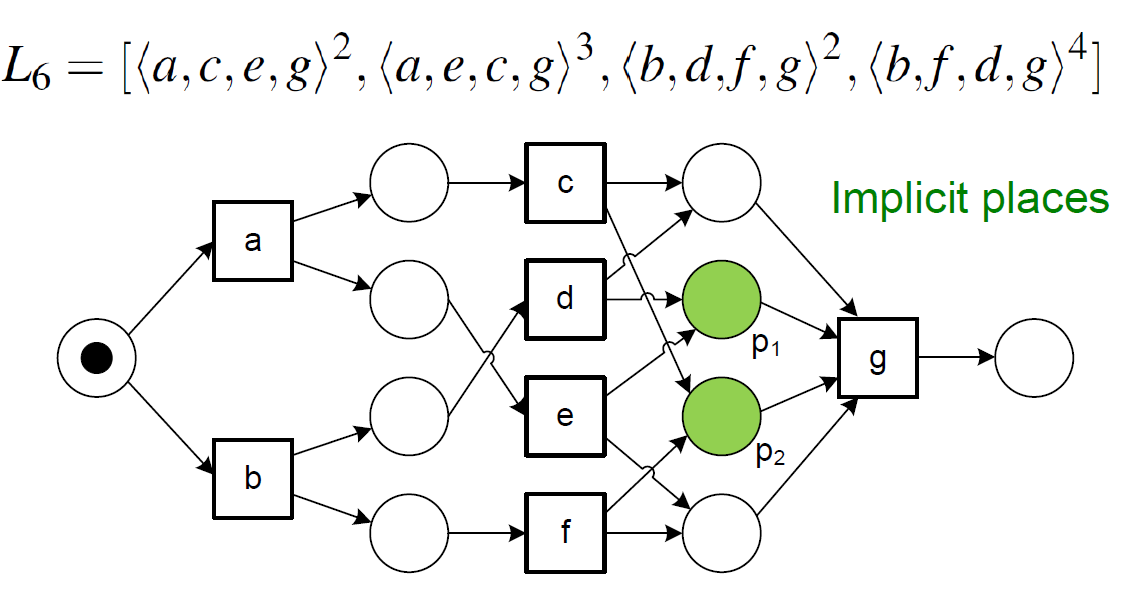
\includegraphics[width=\textwidth]{capitolo 5/5 limit 1 .png}
        \end{center}
        \item \textbf{Loops of length 1:} The algorithm struggles with loops of length 1, where a transition can fire multiple times in succession.
        \begin{center}
            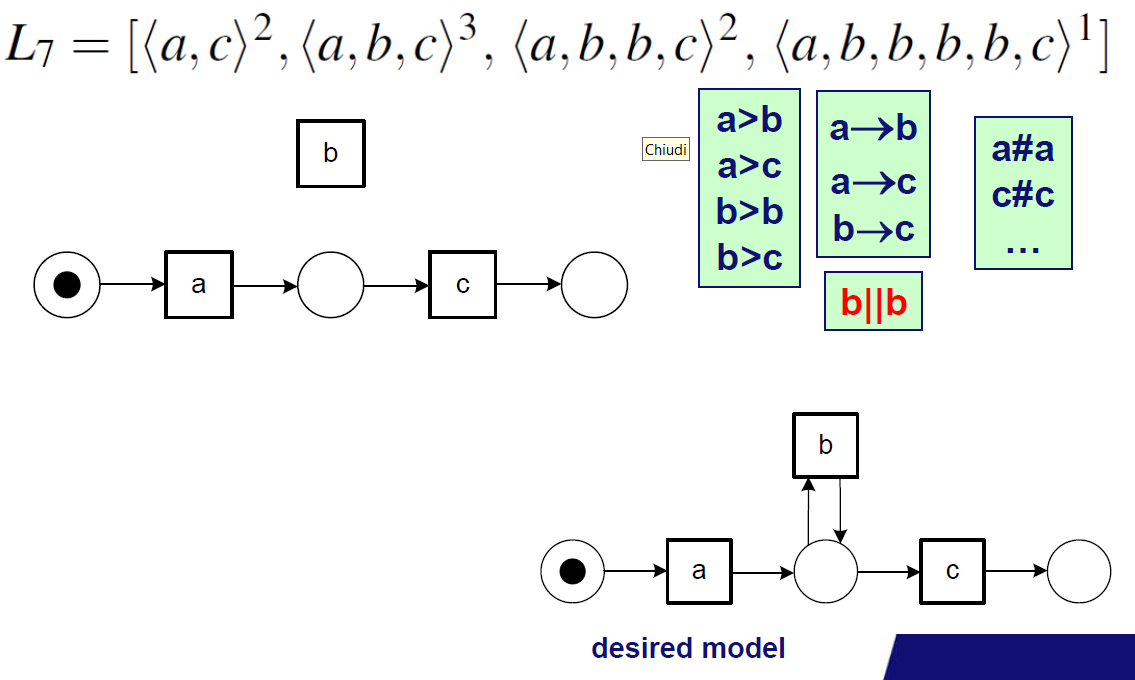
\includegraphics[width=\textwidth]{capitolo 5/5 limit 2.png}
        \end{center}
        \item \textbf{Loops of length 2:} Similarly, the algorithm has difficulty handling loops of length 2, where two transitions alternate repeatedly.
        \begin{center}
            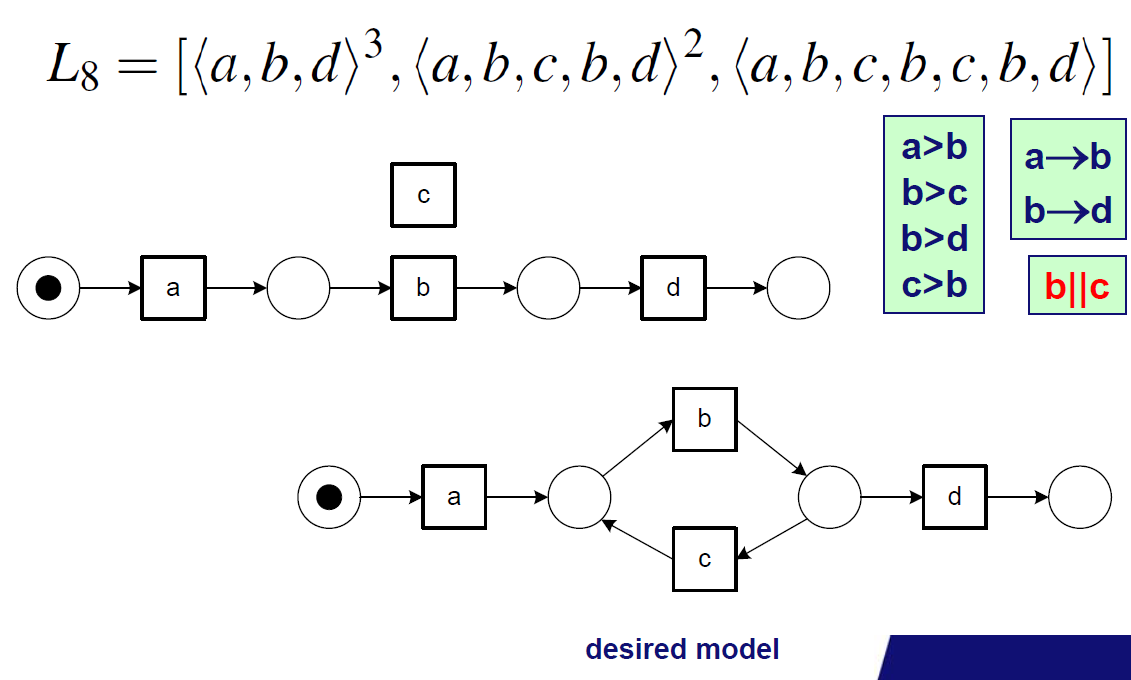
\includegraphics[width=\textwidth]{capitolo 5/5 limit 3.png}
        \end{center}
        \item \textbf{Non-local dependencies:} The algorithm cannot discover non-local dependencies, where the behavior of a transition depends on events that occurred much earlier in the process.
        \begin{center}
            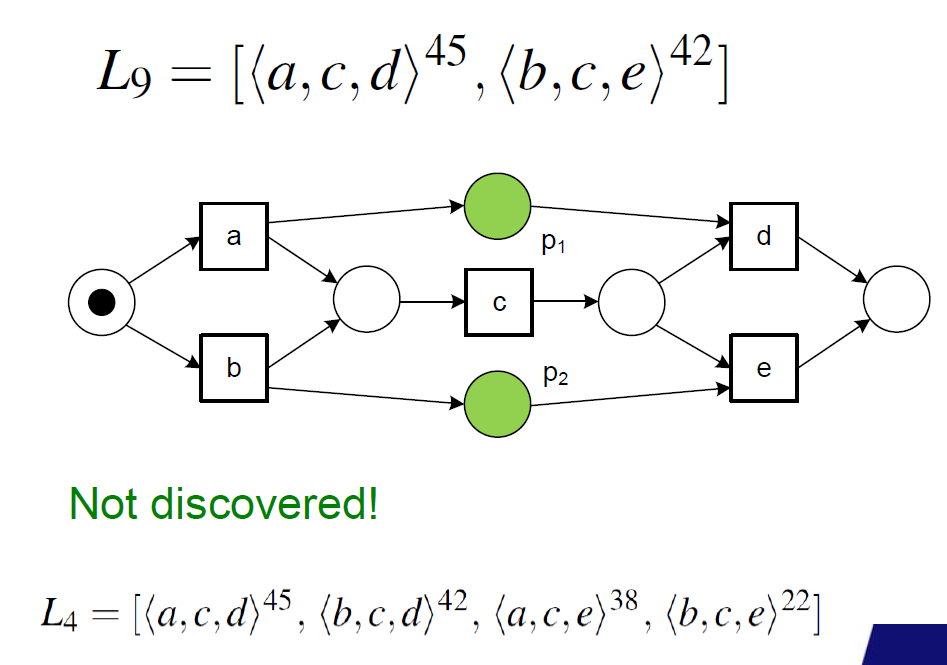
\includegraphics[width=\textwidth]{capitolo 5/5 limit 4.png}
        \end{center}
        \item Some bias is needed because we have to exclude some behaviour such as two equal transitions firing one after the other. 
        \begin{center}
            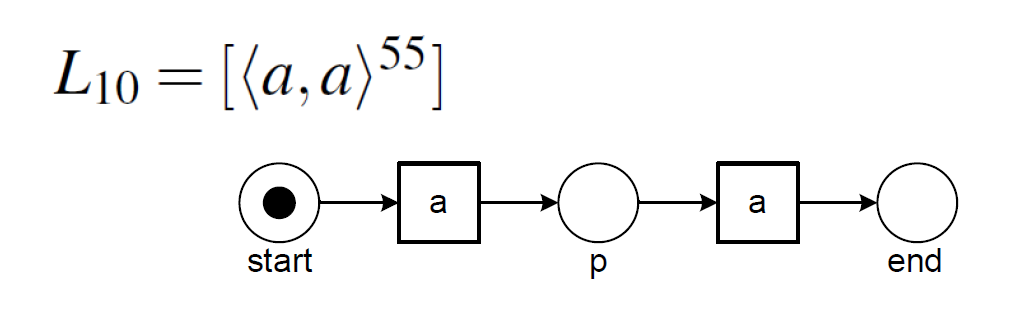
\includegraphics[width=\textwidth]{capitolo 5/5 limit 5.png}
        \end{center}
        \item \textbf{Noise and incompleteness:} Event logs may contain noise, or rare, unrepresentative behavior. Moreover, incomplete logs may not capture all the possible variations of the process. It has to be generalised. 
    \end{itemize}
       
    
    \section{Flower Model}
    
    The \textbf{Flower Model} is an extreme example of an over-generalized process model. It allows any activity to occur at any time, in any order, and still result in a valid process execution. While this model has perfect fitness (i.e., it can replay all the observed traces), it lacks precision and generalization.
    
    \begin{center}
        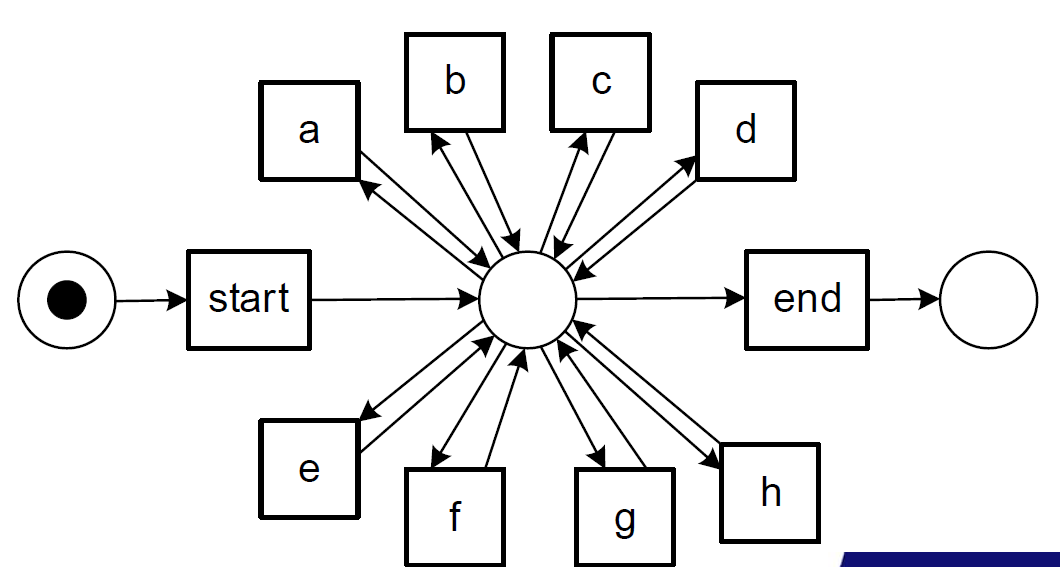
\includegraphics[width=0.5\textwidth]{capitolo 5/5 flower model.png} % Insert image of Flower Model
    \end{center}
    
    \section{Balancing Four Forces in Process Models}
    
    To create an optimal process model, four key forces must be balanced:
    \begin{itemize}
        \item \textbf{Fitness:} The ability of the model to explain the observed behavior in the event log.
        \item \textbf{Generalization:} The ability of the model to handle unobserved but possible behavior, avoiding overfitting.
        \item \textbf{Precision:} The model should not allow behavior that is not present in the log, avoiding underfitting.
        \item \textbf{Simplicity:} The model should be as simple as possible while still capturing the essential behavior of the process.
    \end{itemize}
    
    
    \section{Example: Model Comparison}
    
    Consider the following example of process discovery using a log with multiple traces. The four models below are evaluated based on their \textit{fitness}, \textit{generalization}, \textit{precision}, and \textit{simplicity}.
    
    
    \subsection{Model N1}
    Model N1 has high fitness, precision, generalization, and simplicity. It is an ideal model that balances all four forces well.
    \begin{center}
        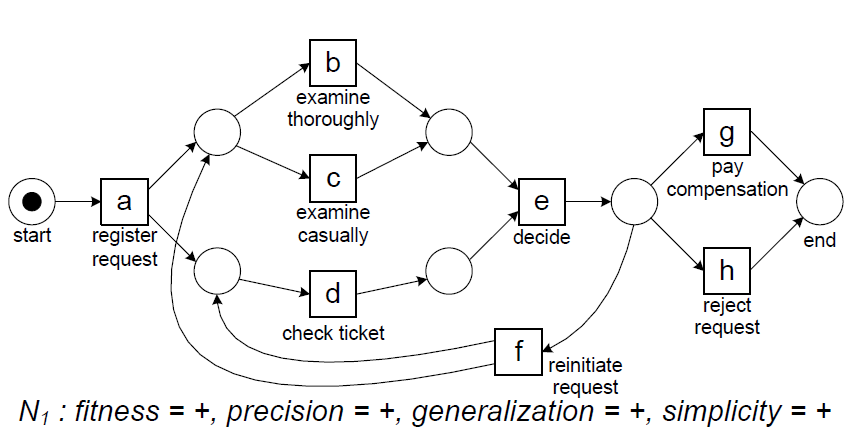
\includegraphics[width=0.5\textwidth]{capitolo 5/5 n1.png} % Insert image of model comparison
    \end{center}
    \subsection{Model N2}
    Model N2 has high precision and simplicity but lacks generalization and fitness. This model may overfit to the observed traces, excluding potential valid behaviors.
    \begin{center}
        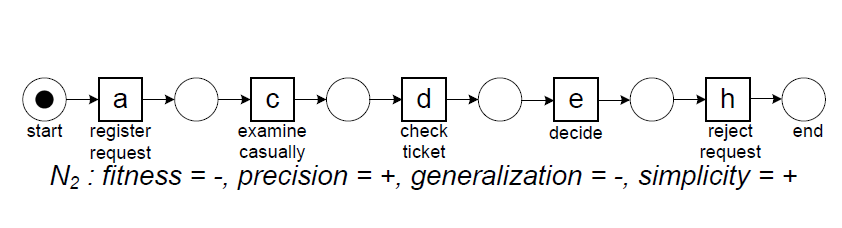
\includegraphics[width=0.5\textwidth]{capitolo 5/5 n2.png} % Insert image of model comparison
    \end{center}
    \subsection{Model N3}
    Model N3 has high fitness and generalization but low precision. This indicates that the model allows too much flexibility, potentially enabling behavior that is not observed in the event log.
    \begin{center}
        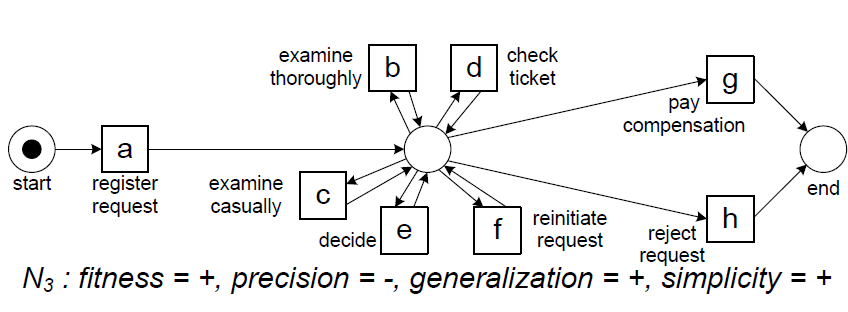
\includegraphics[width=0.5\textwidth]{capitolo 5/5 n3.png} % Insert image of model comparison
    \end{center}
    \subsection{Model N4}
    Model N4 has high fitness and precision but poor generalization. While it accurately reflects the observed traces, it may not handle new or unseen behaviors effectively.
    \begin{center}
        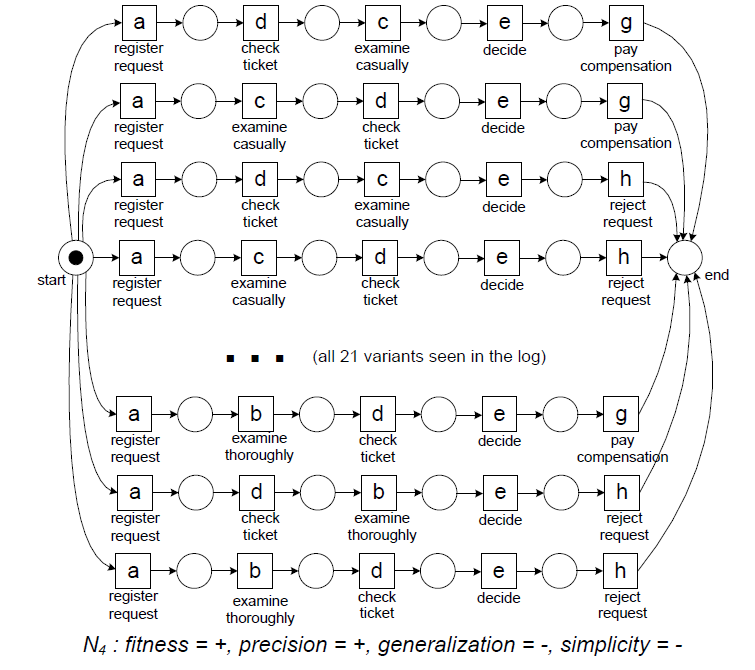
\includegraphics[width=0.5\textwidth]{capitolo 5/5 n4.png} % Insert image of model comparison
    \end{center}
